\begin{quotation}
\ldots
\end{quotation}

\noindent {\em This chapter was derived from a document written by Adam Ferrari and later updated by Alan Batson, Mike Lack, Anita
Jones, and Aaron Bloomfield}

\section{What is a Calling Convention?}

At the end of the previous chapter, we saw a simple example of a
subroutine defined in x86 assembly language. In fact, this subroutine
was quite simple~-- it did not modify any registers except EAX (or
RAX) (which was needed to return the result), and it did not call any
other subroutines. In practice, such simple function definitions are
rarely useful. When more complex subroutines are combined in a single
program, a number of complicating issues arise.  For example, how are
parameters passed to a subroutine? Can subroutines overwrite the
values in a register, or does the caller expect the register contents
to be preserved? Where should local variables in a subroutine be
stored? How should results be returned from functions?

To allow separate programmers to share code and develop libraries for
use by many programs, and to simplify the use of subroutines in
general, programmers typically adopt a common {\em calling
  convention}. The calling convention is simply a set of rules that
answers the above questions without ambiguity to simplify the
definition and use of subroutines. For example, given a set of calling
convention rules, a programmer need not examine the definition of a
subroutine to determine how parameters should be passed to that
subroutine. Furthermore, given a set of calling convention rules,
high-level language compilers can be made to follow the rules, thus
allowing hand-coded assembly language routines and high-level language
routines to call one another.

In practice, even for a single processor instruction set, many calling
conventions are possible.  In this class we will examine and use one
of the most important conventions: the C language calling convention.
Understanding this convention will allow you to write assembly
language subroutines that are safely callable from C and C++ code, and
will also enable you to call C library functions from your assembly
language code.

\section{The C Calling Convention}

The C calling convention is based heavily on the use of the
hardware-supported stack. To understand the C calling convention, you
should first make sure that you fully understand the push, pop, call,
and ret instructions~-- these will be the basis for most of the rules.
In this calling convention, subroutine parameters are passed on the
stack. Registers are saved on the stack, and local variables used by
subroutines are placed in memory on the stack. In fact, this
stack-centric implementation of subroutines is not unique to the C
language or the x86 architecture. The vast majority of high-level
procedural languages implemented on most processors have used similar
calling convention.

The calling convention is broken into two sets of rules. The first set
of rules is employed by the caller of the subroutine, and the second
set of rules is observed by the writer of the subroutine (the
``callee''). It should be emphasized that mistakes in the observance
of these rules quickly result in fatal program errors; thus meticulous
care should be used when implementing the call convention in your own
subroutines.

\section{The Caller's Rules}

The caller should adhere to the following rules when invoking a
subroutine:

\begin{numlist}
\item Before calling a subroutine, the caller should save the contents
  of certain registers that are designated caller-saved. The
  caller-saved registers are r10, r11, and any registers that
  parameters are put into. If you want the contents of these registers
  to be preserved across the subroutine call, push them onto the
  stack.
\item To pass parameters to the subroutine, we put up to six of them
  into registers (in order: rdi, rsi, rdx, rcx, r8, r9).  If there are
  more than six parameters to the subroutine, then push the rest onto
  the stack in {\em reverse order} (i.e. last parameter first)~--
  since the stack grows down, the first of the extra parameters
  (really the seventh parameter) parameter will be stored at the
  lowest address (this inversion of parameters was historically used
  to allow functions to be passed a variable number of parameters).
\item To call the subroutine, use the {\tt call} instruction. This
  instruction places the return address on top of the parameters on
  the stack, and branches to the subroutine code.
\item After the subroutine returns, (i.e. immediately following the
  call instruction) the caller must remove any additional parameters
  (beyond the six stored in registers) from stack.  This restores the
  stack to its state before the call was performed.
\item The caller can expect to find the return value of the subroutine
  in the register RAX.
\item The caller restores the contents of caller-saved registers (r10,
  r11, and any in the parameter passing registers) by popping them off
  of the stack. The caller can assume that no other registers were
  modified by the subroutine.
\end{numlist}

Due to the way the calling convention is structured, it will typically
be the case that some (or most) of these steps will not make any
changes to the stackd.  For example, if there are six or fewer
parameters, then nothing is pushed onto the stack in that step.
Likewise, programmers (and compilers) tyipcally keep the results they
care about out of the caller-saved registers in steps 1 and 6 to
prevent excess pushes and pops.

\section{The Callee's Rules}

The definition of the subroutine should adhere to the following rules:

\begin{numlist}

\item Allocate local variables by using registers or making space on
  the stack.  Recall, the stack grows down, so to make space on the
  top of the stack, the stack pointer should be decremented. The
  amount by which the stack pointer is decremented depends on the
  number of local variables needed. For example, if a local {\tt
    float} and a local {\tt long} (12 bytes total) were required, the
  stack pointer would need to be decremented by 12 to make space for
  these local variables:

\begin{lstlisting}[backgroundcolor=\color{white},frame=trBL,linewidth=3.75in,xleftmargin=2.25in,label={x86-callee-code-2.lst},language={[x86masm]Assembler},caption={x86 callee code, part 2}]
sub rsp, 12
\end{lstlisting}

As with parameters, local variables will be located at known offsets
from the stack pointer.

\item Next, the values of any registers that are designated
  callee-saved that will be used by the function must be saved. To
  save registers, push them onto the stack. The callee-saved registers
  are RBX, RBP, and R12 through R15 (RSP will also be preserved by the
  call convention, but need not be pushed on the stack during this
  step).

  After these three actions are performed, the actual operation of the
  subroutine may proceed.  When the subroutine is ready to return, the
  call convention rules continue:

\item When the function is done, the return value for the function
  should be placed in RAX if it is not already there.

\item The function must restore the old values of any callee-saved
  registers (RBX, RBP, and R12 through R15) that were modified. The
  register contents are restored by popping them from the stack. Note,
  the registers should be popped in the inverse order that they were
  pushed.

\item Next, we deallocate local variables. The easiest way to do this
  is to add to RSP the same amount that was subtracted from it in step
  1.

\item Finally, we return to the caller by executing a {\tt ret}
  instruction. This instruction will find and remove the appropriate
  return address from the stack.

\end{numlist}

If you look at the assembly generated by some compilers, you will see
a few extra commands in there in the callee's prologue:

\begin{lstlisting}[backgroundcolor=\color{white},frame=trBL,linewidth=5.5in,xleftmargin=1.25in,label={x86-callee-code-2.lst},language={[x86masm]Assembler},caption={x86 extraneous codedd}]
push rbp       ; at the start of the callee
mov rbp, rsp
...
pop rbp        ; just before the ending 'ret'
\end{lstlisting}

This code is unnecessary, and is a hold-over from the 32-bit calling
convention.  You can tell the compiler to not include this code by
invoking it with the {\tt -fomit-frame-pointer} flag.

It might be noted that the callee's rules fall cleanly into two halves
that are basically mirror images of one another. The first half of the
rules apply to the beginning of the function, and are therefor
commonly said to define the {\em prologue} to the function. The latter
half of the rules apply to the end of the function, and are thus
commonly said to define the {\em epilogue} of the function.

\section{Calling Convention Example}

The above rules may seem somewhat abstract on first examination. In practice, the rules
become simple to use when they are well understood and familiar. To start the process of better
understanding the call convention, we now examine a simple example of a subroutine call and a
subroutine definition.

\begin{figure}[h!]
\lstinputlisting[caption={Example function call, caller's rules obeyed},label={x86-caller-example-1.s.lst},backgroundcolor=\color{white},frame=trBL,linewidth=6in,xleftmargin=0.75in,language={[x86masm]Assembler}]{x86-64bit/code/caller-example-1.s}
\end{figure}


In Listing~\ref{x86-caller-example-1.s.lst} a sample function call is
depicted. The three parameters are put into the parameter passing
registers; if there were more than 6, then the additional ones would
be pushed onto the stack in reverse order.  The call instruction is
used to jump to the beginning of the subroutine in anticipation of the
fact that the subroutine will use the ret instruction to return when
the subroutine completes. When the subroutine returns, the parameters
must be removed from the stack. A simple way to do this is to add the
appropriate amount to the stack pointer (since the stack grows down).
Finally, the result is available in RAX.

Next up is the caller's rules. An example subroutine implementation
that obeys the callee's rules is depicted in
Listing~\ref{x86-callee-example-1.s.lst}. The subroutine prologue
performs the standard actions of allocating local variables by
decrementing the stack pointer, and saving register values on the
stack.

\begin{figure}[h!]
\lstinputlisting[caption={Example function definition, callee's rules obeyed},label={x86-callee-example-1.s.lst},backgroundcolor=\color{white},frame=trBL,linewidth=6.9in,xleftmargin=0.15in,language={[x86masm]Assembler}]{x86-64bit/code/callee-example-1.s}
\end{figure}

In the body of the subroutine we can how the local variables are
accessed.  The prologue put 24 bytes of ``stuff'' onto the stack:
three 8 byte values.  The first was the local variable (via the {\tt
  sub rsp, 8} call).  The second was the rbx backup, and the third was
the rbp backup.  Thus, the stack pointer is now 16 bytes below the
local variable, as two 8 byte ``things'' have been pushed onto the
stack since the local variable was allocated.  Thus, to access the
local variable, one uses {\tt [rsp+16]}, as seen throughout the code.

The function epilogue, as expected, is basically a mirror image of the
function prologue. The caller's register values are recovered from the
stack, the local variables are deallocated by resetting the stack
pointer, and the {\tt ret} instruction is used to return to the
appropriate code location in the caller.

A good way to visualize the operation of the calling convention is to
draw the contents of the nearby region of the stack during subroutine
execution. Figure~\ref{x86-activation-record.fig} depicts the contents
of the stack during the execution of the body of myFunc (myFunc is
depicted in Listing~\ref{x86-callee-example-1.s.lst}). Notice, lower
addresses are depicted lower in the figure, and thus the ``top'' of
the stack is the bottom-most cell. This corresponds visually to the
intuitive statement that the x86 hardware stack ``grows down.'' The
cells depicted in the stack are 64-bit wide memory locations, thus the
memory addresses of the cells are 4 bytes apart. From this picture we
see clearly why the first parameter resides at an offset of 8 bytes
from the base pointer. Above the parameters on the stack (and below
the base pointer), the call instruction placed the return address,
thus leading to an extra 4 bytes of offset from the base pointer to
the first parameter.

\begin{figure}[h]
\centering
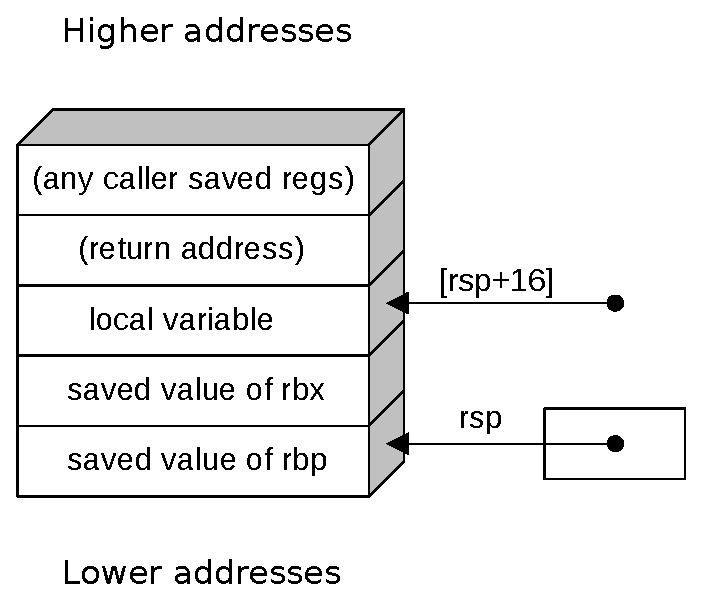
\includegraphics[width=4in]{x86-64bit/x86-activation-record.pdf}
\caption{A picture of the stack in memory during the execution of the body of myFunc}
\label{x86-activation-record.fig}
\end{figure}

The assembly code for {\tt myFunc()} was shown above in
Listing~\ref{x86-callee-example-1.s.lst}. The C++ code to call that
subroutine is shown in
Listing~\ref{x86-callee-example-main.cpp.lst}.

\begin{figure}[h!]
\lstinputlisting[caption={Example C++ code to invoke a 3-parameter x86 subroutine},label={x86-callee-example-main.cpp.lst},backgroundcolor=\color{white},frame=trBL,linewidth=6.9in,xleftmargin=0.15in,language=C++]{x86-64bit/code/callee-example-main.cpp}
\end{figure}




